/\chapter{Crittografia Visuale}

L'idea della \textbf{Crittografia Visuale} nasce nel 1994 da un'intuizione dei crittografi Naor e Shamir. L'obiettivo di questo sistema è prendere un'immagine segreta e dividerla in due immagini apparentemente casuali, chiamate \textbf{share} (condivisioni), che fungono l'una da chiave e l'altra da crittogramma. 

La particolarità di questo approccio è che, preso singolarmente, uno share non rivela assolutamente alcuna informazione a un potenziale attaccante. L'unico modo per decifrare e rivelare l'immagine originale è andare a sovrapporre fisicamente (o digitalmente) la chiave al crittogramma.

Un classico esempio è il seguente:
\begin{figure}[H]
    \centering
    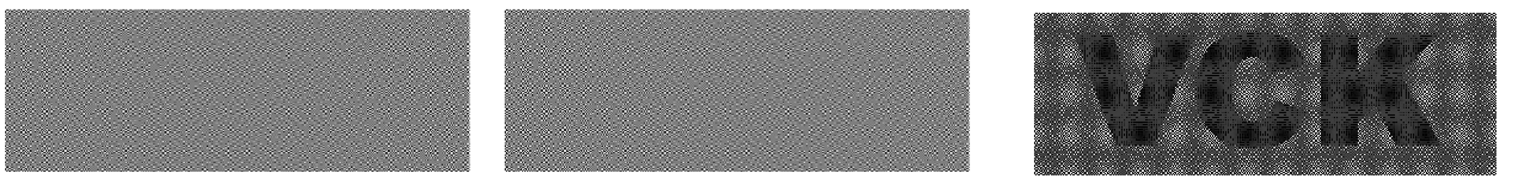
\includegraphics[width=0.5\linewidth]{Images/capitolo_3/esempio_vck.png}
    \caption{Esempio di sovrapposizione di due share.}
\end{figure}

Come possiamo notare, se spostiamo uno dei due blocchi sopra l'altro, appare in chiaro la scritta "VCK". In pratica, in questo tipo di crittografia non è richiesta alcuna potenza di calcolo: \textbf{è il nostro occhio a fungere da decoder}.

\section*{Applicazioni e Funzionamento Logico}
Questo sistema trova molte applicazioni interessanti, specialmente nel contesto bancario. Una banca, ad esempio, può spedire fisicamente lo share "chiave" (stampato su un foglio lucido trasparente) al cliente e pubblicare lo share "crittogramma" sulla propria pagina web. In questo modo, solo il cliente legittimo potrà sovrapporre il suo lucido allo schermo per leggere un PIN o una password monouso, rendendo le intercettazioni di rete del tutto inutili.

\subsection*{L'Implementazione tramite Matrici $2 \times 2$}
A livello logico, il sistema utilizza uno schema che riprende i concetti del \textbf{One-Time Pad} (il cifrario perfetto) e sfrutta le proprietà dell'operazione \textbf{XOR} (OR esclusivo). Si predilige l'uso logico dello XOR rispetto al classico OR perché quest'ultimo comporta una \textbf{perdita di informazione}, mentre lo XOR ci garantisce la perfetta decodifica del messaggio. Bisogna sempre ricordare che lo XOR è una delle codifiche più robuste a patto che la chiave abbia la stessa lunghezza del messaggio e che questa venga utilizzata una sola volta. Se fosse riutilizzata, allora avremmo che si potrebbe estrarre la chiave e, dunque, decodificare ogni messaggio.

Per implementare questa logica graficamente, ogni singolo pixel dell'immagine originale viene espanso in due matrici di dimensione $2 \times 2$ (una per il primo share e una per il secondo share). Ognuna di queste sottomatrici è composta da esattamente 2 pixel neri e 2 pixel bianchi (o trasparenti).

\begin{figure}[H]
    \centering
    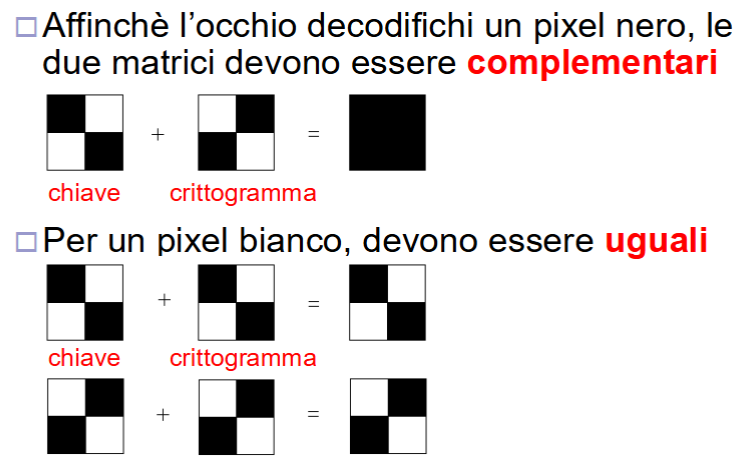
\includegraphics[width=0.5\linewidth]{Images/capitolo_3/matrice_2x2.png}
    \caption{Espansione di un singolo pixel in sottomatrici $2 \times 2$.}
\end{figure}

Il trucco risiede nella loro \textbf{sovrapposizione} (overlay):
\begin{itemize}
    \item Se i due share hanno i pixel neri disposti in posizioni \textit{diverse} (complementari), la loro sovrapposizione coprirà tutti e quattro gli spazi della matrice+ $2 \times 2$, restituendo un macro-pixel \textbf{completamente nero}.
    \item Se i due share hanno i pixel neri nella \textit{stessa} posizione, la sovrapposizione lascerà scoperti i due spazi bianchi. Il risultato sarà un macro-pixel per metà nero e per metà bianco.
\end{itemize}

\begin{figure}[H]
    \centering
    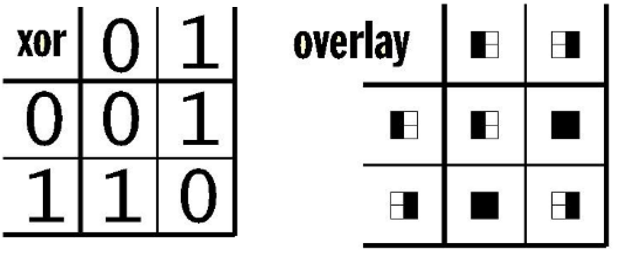
\includegraphics[width=0.5\linewidth]{Images/capitolo_3/differenza_xor_overlay.png}
    \caption{L'effetto visivo della sovrapposizione (XOR visivo).}
\end{figure}

Nonostante un pixel per metà nero e per metà bianco non sia tecnicamente "bianco puro", l'occhio umano interpreterà questo contrasto come una sfumatura di grigio. Questo stacco netto tra il nero totale e il grigio chiaro permette al nostro cervello di distinguere chiaramente la forma dell'immagine nascosta, facendo funzionare l'overlay grafico esattamente come una decodifica XOR. 

In genere, dunque, quello che cerchiamo è un contrasto sufficientemente alto da far sì che l'occhio riesca a distinguere chiaramente la "scritta" dallo "sfondo". Sebbene sia teoricamente possibile rappresentare non solo bianco e nero puro, ma anche 3 scale di grigio intermedie con una semplice matrice $2 \times 2$, questo abbasserebbe drasticamente il contrasto visivo, rendendo il messaggio finale molto difficile da decifrare a occhio nudo.

Per questo motivo, nel caso in cui volessimo rappresentare 4 scale di grigio ben distinte mantenendo una buona leggibilità, avremmo bisogno di espandere i pixel su una matrice $3 \times 3$, gestendola nel seguente modo:

\begin{figure}[H]
    \centering
    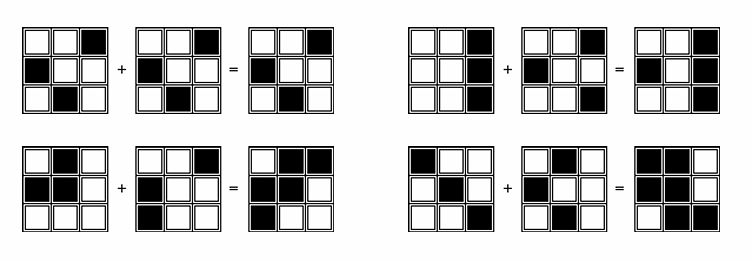
\includegraphics[width=0.5\linewidth]{Images/capitolo_3/matrice_3x3.png}
\end{figure}

Anche in questo caso, la regola generale è che all'aumentare dei pixel "accesi" possiamo rappresentare più sfumature, ma paghiamo il prezzo di un contrasto sempre minore, che rende più faticosa la decodifica visiva dello share.

Un'altra nota teorica fondamentale riguarda la \textbf{perfetta sicurezza} del sistema. Proprio come in One-Time Pad, affinché lo schema sia inattaccabile, ogni share crittografico generato deve essere perfettamente equiprobabile. Cosicché, analizzando un singolo share isolato, un attaccante non possa dedurre alcuna informazione statistica sull'immagine originale sfruttando attacchi probabilistici.

L'algoritmo di codifica generico si può quindi riassumere in due fasi:
\begin{enumerate}
    \item Per ogni pixel dell'immagine segreta, si sceglie \textbf{a caso} la matrice da associargli per il primo share (la chiave). Essendo la scelta puramente casuale, questo primo share apparirà visivamente come puro rumore bianco.
    \item Successivamente, si costruisce il secondo share (il crittogramma) guardando il pixel corrispondente nell'immagine di partenza. Se il pixel originale è nero, per il secondo share si sceglie la matrice \textbf{complementare} a quella usata nella chiave; se il pixel originale è bianco, si sceglie la \textbf{stessa identica} matrice della chiave.
\end{enumerate}

Così facendo, la sovrapposizione fisica dei due share darà come risultato nero totale nei punti in cui le matrici sono complementari (pixel originali neri) e un grigio composto per metà da spazi bianchi nei punti in cui le matrici sono identiche (pixel originali bianchi), riproducendo l'immagine corretta.


Esistono, inoltre, altri schemi di cifratura visuale come, ad esempio gli \textbf{schemi a soglia} in cui è necessario avere un certo numero di share totali per ottenere l'immagine originale. Allo stesso modo, esistono degli \textbf{schemi a gruppi di accesso} in cui è possibile decifrare una certa immagine solo se si possiedono contemporaneamente degli specifici gruppi di share. 